\chapter{Development Process}

\section{Initial setup}
The initial project setup consists of various steps including setting up the
local development environment, Python and its dependencies and finally the
initial Django project template. Django project can be initialized using the
command \texttt{django-admin startproject mysite}. The command will create a
new directory named \texttt{mysite} in your current directory. It represents
the Django project. Once the project has been initialized, we need to create
a new application within the project by the command
\texttt{python manage.py startapp appname}. This will create a new directory
inside your project directory representing a Django application.

Once the application has been initialized, we can move towards the actual
development of the application. This process involves several steps including
creating models, views, serializers, services etc. But before that it is
important to setup the project settings correctly. You can select the database
driver of your choice and modify the \texttt{settings.py} file in your project
directory.

\section{Create models}
As mentioned previously before, models represent the database tables. These
models can be defined in seperate files or can be defined in a single file
named \texttt{models.py} as required. Before starting to write the actual
implementation it is critical to design and write the database schema first.
Django provides you with an inbuilt \texttt{Model} class which you can extend
to write you own models. Most of the methods in the \texttt{Model} class are
reusable and hence we don't have to write custom methods for every class.

\begin{pythoncode}
# models/turtlemint_model.py

class TurtlemintModel(models.Model):
    """
    Model representing Turtlemint meta model.
    """
    key = models.CharField(max_length=100, unique=True, blank=True)
    name = models.CharField(max_length=100)
    description = models.TextField(max_length=100)
    logo = models.CharField(max_length=200, null=True, blank=True)
    home_url = models.CharField(max_length=200, null=True)
    support_email = models.EmailField(blank=True, null=True)
    ...
\end{pythoncode}

\begin{pythoncode}
# models/turtlemint_insurer_model.py
    
class InsurerModel(models.Model):
    """
    Model representing insurer meta model.
    """
    key = models.CharField(max_length=100, unique=True, blank=True)
    name = models.CharField(max_length=100)
    associated_vertical = models.CharField(max_length=200, null=True)
    logo = models.CharField(max_length=200, null=True, blank=True)
    home_url = models.CharField(max_length=200, null=True, blank=True)
    support_email = models.EmailField(blank=True, null=True)
    ...
\end{pythoncode}

To make reflect these models into our database we need to create Django
migrations. These migrations can be created using the command
\texttt{python manage.py makemigrations}. This would create a new directory
inside you app representing the database queries. Internally, Django parses
the changes made to the models into their equivalent database queries. These
created migrations are then ran using the command
\texttt{python manage.py migrate} to reflect them in your database.

\section{Create serializers}
Serializers allow complex data such as querysets and model instances to be
converted to native Python datatypes that can then be easily rendered into
JSON, XML or other content types. Serializers also provide deserialization,
allowing parsed data to be converted back into complex types, after first
validating the incoming data.

Every models should have its own serializer, representing the construction of
the JSON object throught the model fields. Serializers are extremely useful
to return the JSON object instantly without having to construct it manually.
Django allows us to define the fields we want the serializer to construct the
JSON with. Also, we can have multiple serializers for a model if we want a
separate response based on the request.

An example of serializer can be given as below:
\begin{pythoncode}
class TurtlemintModelSerializer(serializers.ModelSerializer):
    """
    Serializer for the TurtlemintModel.
    """
    class Meta:
        model = TurtlemintModel
        fields = ['id', 'key', 'name', 'description', 'language'...]
\end{pythoncode}

\section{Add CRUD operations}
Every model should have its own each of CRUD methods. These methods will be
commonly shared and used by the views and business logic. Also these functions
should be unittestable to make sure that they are doing exactly what is
intended of them. Hence it is critical that these methods should be an early
part of the development process.

\section{Add views}
Views take care of accepting the request and returning the appropriate
response. These are defined inside the \texttt{views} module and can be split
into various files and classes. Views can be written in two ways, having a
separate class to handle all requests including GET, POST, DELETE, etc for a
single endpoint or to have indivitual view methods for each type of request.
Django supports both ways equally and hence any method should suffice based
on the development need.

Examples of views:
\begin{pythoncode}
class TurtlemintView(APIView):
    """
    Turtlemint view.
    """
    def get(self, request):
        return Response(Turtlemint.get_data(request.data),
                        status_code=status.HTTP_200_OK)
    def post(self, request):
        responseTurtlemint.update(request.data)
        if response['success']:
            return Response(response, status_code=HTTP_200_OK)
        return Response(response, status_code=HTTP_400_BAD_REQUEST)
\end{pythoncode}

To make this operational for an endpoint, we need to add an entry in
\texttt{urls.py} file for the same.

\begin{pythoncode}
# urls.py
urlpatterns = [
    ...
    path('api/v1/turtlemint/meta', TurtlemintView.as_view()),
    ...
]
\end{pythoncode}

The views also link to the business logic for that API, this will be covered
in the next chapter as a part of Turtlemint and its requirements.

\section{API testing}
The APIs can be manually tested using any framework like Postman. Django also
provides a nice UI to be able to send requests. At turtlemint we've a culture
of using Postman extensively for API testing and we've followed the same.
Although, apart from the Postman tests it is also necessary to construct
unittests and view tests using Django's \texttt{TestCase} class.

\subsection{Unittests}
Django provides an extended version of \texttt{unittest.TestCase} class which
automatically creates a test database and destroys it at the end of test
execution cycle. Also every test is ran as a separate transaction hence
allowing the database to rollback automatically once some error is encountered
in the tests.

As per the default behaviour of unittest, every test file should start with
\texttt{test} prefix and should correctly represent the file under testing.
Tests can be written as a part of a class which may include \texttt{setUp}
and \texttt{taildown} function to represent to initate, and clear some process
at the start and the end of the test execution.

\begin{pythoncode}
class TestTurtlemintModel(TestCase):
    def setUp(self):
        # Run something before running the testcase
        self.model = TurtlemintModel
    def test_get_records_count(self):
        # Get the output from the method under test
        result = get_records_count(self.model)
        self.assertEqual(result, 1) # 1 representing expexted result
\end{pythoncode}

\subsection{Postman tests}
Unittests are always preferred, but for some reason if we need some sort of
integration tests then postman tests can be written. Postman is an application
used for API collection management. It introduces a lot of features including
one to write tests for the API collections. For every request you can mock
the expected response and check if the response is correct or not. Although
this might be helpful in some cases, we initially wrote some tests here but
later due to introduction of unittests we dropped this process.

\begin{figure}
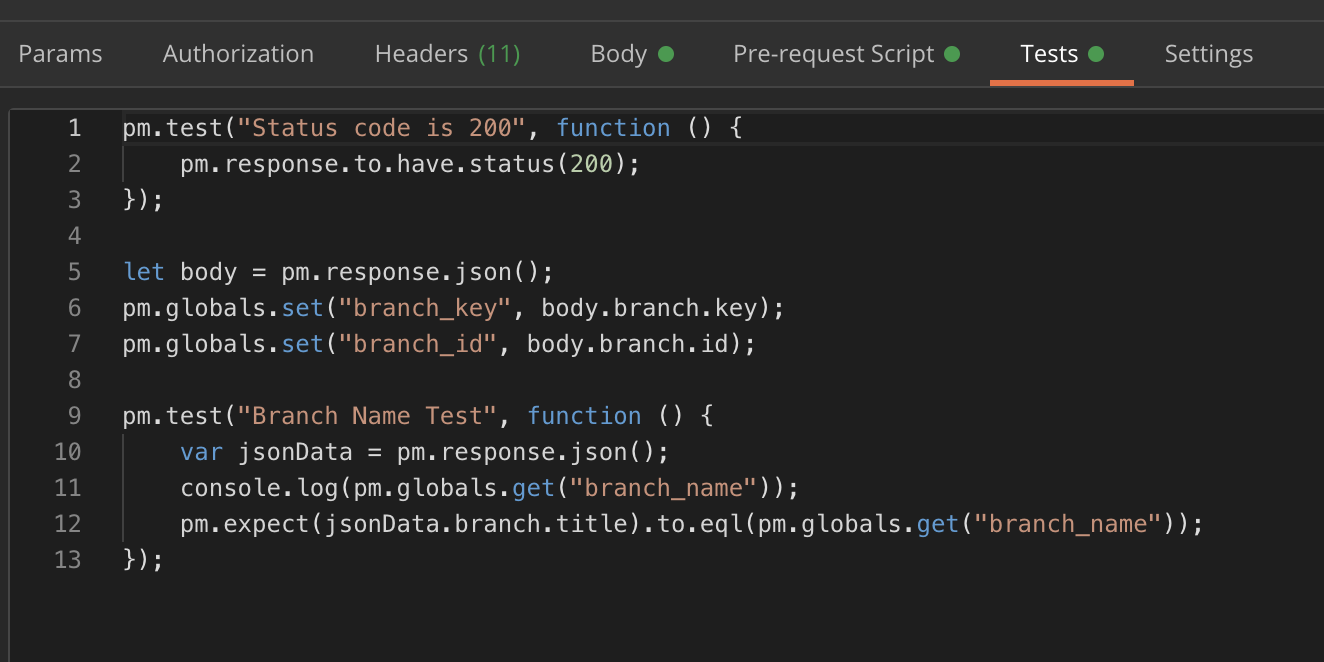
\includegraphics[width=\textwidth]{ch4/postman_test.png}
\caption{Sample Postman testcase}
\end{figure}
